\documentclass{beamer}
\usefonttheme{professionalfonts}  % serif math

\iffalse
\usepackage{pgfpages}
\setbeameroption{show notes}
\setbeameroption{show notes on second screen=right}
% pdfpc slajdovi.pdf --notes=right
\fi

\usepackage[scaled]{beramono}				% sans-serif monospace
% font
\renewcommand{\familydefault}{\sfdefault}  % sans-serif main

%\usepackage{arev}
%\usepackage[cm]{sfmath}  % bolje nego mathastext
%\SetSymbolFont{largesymbols}{normal}{OMX}{iwona}{m}{n}

%\usepackage[italic]{mathastext}  % sfmath je bolje (manji indeksi)


%\usepackage{inconsolata}					% sans-serif monospace
\usepackage[scaled]{beramono}				% sans-serif monospace


%\usepackage[math]{iwona}
%\usepackage[math]{kurier}
%\usepackage[T1]{fontenc}  % accented characters, copy from pdf, ...

\raggedright						% bez desnog poravnavanja

\usepackage{caption}
\captionsetup{%
	justification=raggedright,
}
\setlength{\parindent}{1em}	 % uvlačenje ulomaka
\usepackage{indentfirst}	 % uvlačenje prvog ulomka
\setlength{\parskip}{0.5em}	 % razmak između ulomaka

\usepackage{listings}  % listings
\renewcommand{\lstlistingname}{Ispis}

\usepackage[multiple]{footmisc}	 % višestruke fusnote

\usepackage[hidelinks]{hyperref}
\renewcommand*{\UrlFont}{\footnotesize}

% colors

\usepackage{xcolor}
\usepackage{color}

\hypersetup{
	colorlinks,
	linkcolor={blue!50!green!50!black},  % xcolor package
	citecolor={green!40!black},
	urlcolor={blue!75!green!30!black}
}
\definecolor{bluekeywords}{rgb}{0.13,0.13,1}  % color package
\definecolor{greencomments}{rgb}{0,0.5,0}
\definecolor{redstrings}{rgb}{0.9,0,0}

\let\emph\relax
\DeclareTextFontCommand{\emph}{\bfseries}

\newtheorem{theorem}{Teorem}[section]
\newtheorem{definition}{Definicija}[section]

\usepackage{enumitem}  % \begin{enumerate}[topsep=0pt,itemsep=0pt,partopsep=0pt]

%%text%%
\iftrue
	\raggedright						% bez desnog poravnavanja
	\raggedbottom
	\usepackage{caption}
	\captionsetup{%
		justification=raggedright,
	}
	\usepackage{etoolbox}
	\makeatletter
	\patchcmd{\@dottedtocline}
	{\rightskip\@tocrmarg}
	{\rightskip\@tocrmarg plus 4em \hyphenpenalty\@M}
	{}{}
	\makeatother
	\setlength{\parindent}{1em}	 % uvlačenje ulomaka
	\usepackage{indentfirst}	 % uvlačenje prvog ulomka
	\setlength{\parskip}{0.5em}	 % razmak između ulomaka
	
	\usepackage[multiple, bottom]{footmisc}	 % višestruke fusnote, poslije slika/tablica
	
	\renewcommand*{\UrlFont}{\footnotesize}
	
	% colors	
	\iffalse
	\usepackage{xcolor}
	\usepackage{color}
	\hypersetup{
		colorlinks,
		linkcolor={blue!60!green!50!black},  % xcolor package
		citecolor={green!40!black},
		urlcolor={blue!75!green!30!black}
	}
	\definecolor{bluekeywords}{rgb}{0.13,0.13,1}  % color package
	\definecolor{greencomments}{rgb}{0,0.5,0}
	\definecolor{redstrings}{rgb}{0.9,0,0}
	\fi
	
	\DeclareTextFontCommand{\textbf}{\bfseries}
\fi
%%%%%%%%
% redefinition of left and right to make spacing consistent
\let\originalleft\left
\let\originalright\right
\def\left#1{\mathopen{}\originalleft#1}
\def\right#1{\originalright#1\mathclose{}}

\usepackage{amsmath}
\usepackage{mathtools}  % \coloneqq
%\usepackage{bm}
%\usepackage[utopia]{mathdesign}
\usepackage[OMLmathsfit]{isomath}  % \DeclareMathAlphabet ...
%\usepackage[bbgreekl]{mathbbol}

\usepackage{mathtools}  % smashoperator
\usepackage{commath}  % calculus, perentheses
\usepackage{stmaryrd}  % \llbracket for \rrbracket, ...

%\usepackage[croatian]{babel}		% teorem
%\newtheorem{definition}{Definicija}[section]
%\newtheorem{theorem}{Teorem}[section]
%\newtheorem{corollary}{Korolar}[theorem]

\DeclareMathAlphabet{\mathbbmsl}{U}{bbm}{m}{sl}
\DeclareMathAlphabet{\mathbbmb}{U}{bbm}{b}{it}
\DeclareMathAlphabet{\mathbbmssit}{U}{bbmss}{m}{it}


% common set?, distribution
\newcommand{\commset}[1]{\mathbbmb{#1}}
\newcommand{\distrib}[1]{\mathcal{#1}}

% sans-serif blackboard-bold
\newcommand{\mathsfbbit}[1]{\mathbbmssit{#1}}

% variable
\let\vec\relax
\let\set\relax
\newcommand{\vec}[1]{\mathbfit{#1}}
\newcommand{\mat}[1]{\vec{#1}}
\newcommand{\ten}[1]{\vec{#1}}
\newcommand{\set}[1]{\mathbbmsl{#1}}

% constant
\newcommand{\const}[1]{\mathrm{#1}}
\newcommand{\cvec}[1]{\mathbf{#1}}
\newcommand{\cmat}[1]{\cvec{#1}}
\newcommand{\cten}[1]{\cvec{#1}}
\newcommand{\cset}[1]{\mathbb{#1}}

% random variable
\newcommand{\rvar}[1]{{\color{blue!70!black}\mathsfit{#1}}}
\newcommand{\rvec}[1]{{\color{blue!70!black}\mathsfbfit{#1}}}
\newcommand{\rmat}[1]{\rvec{#1}}
\newcommand{\rten}[1]{\rvec{#1}}
\newcommand{\rset}[1]{{\color{blue!70!black}\mathsfbbit{#1}}}

% linear algebra
\newcommand{\transpose}{\mathsf T}

% calculus - commath: od, pd, md, dif
% parentheses - commath: del, cbr, sbr, envert, enVert

% named functions
\DeclareMathOperator{\softplus}{softplus}
\DeclareMathOperator{\softmax}{softmax}
\DeclareMathOperator{\logistic}{\sigma}
\DeclareMathOperator{\sgn}{sgn}
\DeclareMathOperator{\diag}{diag}

% operators
\DeclareMathOperator*{\argmin}{arg\,min} % thin space
\DeclareMathOperator*{\argmax}{arg\,max}
\DeclareMathOperator*{\E}{{\rm I\kern-.282em E}}
\DeclareMathOperator*{\D}{{\rm I\kern-.282em D}}
\DeclareMathOperator*{\Cov}{Cov}
\let\H\relax
\DeclareMathOperator*{\H}{{\rm H\kern-.8em H}}
\DeclareMathOperator*{\Dklsym}{D_{\mathrm{KL}}}

% bracket operators
\newcommand{\enangle}[1]{\mathinner{\left\langle{#1}\right\rangle}}
\newcommand{\enbbracket}[1]{\mathinner{\left\llbracket{#1}\right\rrbracket}}
\newcommand{\braket}[2]{\enangle{{#1}|{#2}}}

% parentheses from commath redefined to improve spacing because (left and right were redefined)
\renewcommand{\del}[1]{\left(#1\right)}
\renewcommand{\sbr}[1]{\left[#1\right]}
\renewcommand{\cbr}[1]{\left\{#1\right\}}
\renewcommand{\intoo}[1]{\mathinner{\del{#1}}}
\renewcommand{\intcc}[1]{\mathinner{\sbr{#1}}}
\renewcommand{\intco}[1]{\mathinner{\left[#1\right)}}
\renewcommand{\intoc}[1]{\mathinner{\left(#1\right]}}

% special
\newcommand{\funcdef}[3]{#1 \colon #2 \to #3}
\newcommand{\Dkl}[2]{\Dklsym\del{#1\;\middle\|\;#2}}
\newcommand{\C}{\cset{C}}
\newcommand{\R}{\cset{R}}
\newcommand{\Z}{\cset{Z}}
\newcommand{\N}{\cset{N}}
\newcommand{\dirac}{\delta}
\newcommand{\ind}[2]{#1_{\sbr{#2}}}

% operators
\newcommand{\bidot}{\mkern1.5mu{..}\mkern1.5mu}
\newcommand\sheq{\mkern1.5mu{=}\mkern1.5mu}
%\renewcommand{\dots}{...}
\usepackage{booktabs}  % from the tamplate; table quality enhancement

\usepackage{multirow}
\usepackage{tabularx}

\newcolumntype{P}[1]{>{\raggedright\let\newline\\\arraybackslash\hspace{0pt}}p{#1}}

\renewcommand{\arraystretch}{1.4}
%\usepackage{floatrow} 				% centriranje svih slika
\usepackage{float}					% figure [H]
\usepackage{graphicx} 				% includegraphics
\usepackage{caption}			% subfigure
\usepackage{subcaption}			% subfigure
\usepackage[export]{adjustbox} 	% http://ctan.org/pkg/adjustbox

\usepackage[section]{placeins}  % [section] for \FloatBarrier before every section 

\graphicspath{ {./figures/} }		% mapa sa slikama
%\let\oldincludegraphics\includegraphics
%\renewcommand{\includegraphics}[2][]{\oldincludegraphics[#1,max width=0.9\linewidth]{#2}}

%\usepackage{flafter} % floats after the first reference

\usepackage{tikz} 					% dijagrami
\usepackage{pgfplots}
\usetikzlibrary{fit,automata,arrows,positioning,calc,petri,topaths,arrows.meta}

%\usetikzlibrary{external}
%\tikzexternalize[prefix=figures/tikz/, shell escape=-enable-write18]
%TexStudio Configuration\commands\pdflatex:
%"pdflatex.exe -src -interaction=nonstopmode --shell-escape %.tex

\pgfplotsset{every axis/.append style={
		axis x line=middle,    	% put the x axis in the middle
		axis y line=middle,    	% put the y axis in the middle
		axis line style={->},  	% arrows on the axis
		xlabel={$x$},          	% default put x on x-axis
		ylabel={$y$},          	% default put y on y-axis
		samples=100,
		axis equal,
}} % axis style

\tikzset{
	>={Triangle[length=1.8mm,width=1.2mm]},
	dedge/.style={arrows=->, black, thick},
}
% PGMs
\tikzstyle{textnode} = [minimum size=5mm, node distance=9mm]
\tikzstyle{pnode} = [circle, minimum size=10mm, thick, draw=black, node distance=9mm]
\tikzstyle{greypnode} = [pnode, fill=black!5]
% https://github.com/jluttine/tikz-bayesnet
\tikzstyle{wrap} = [inner sep=0pt, fit=#1]
\tikzstyle{plate} = [draw, rectangle, rounded corners=0.5ex, thick, fit=#1]
\tikzstyle{caption} = [font=\footnotesize, node distance=0]
\tikzstyle{plate caption} = [caption, node distance=0, inner sep=0pt,
below left=5pt and 0pt of #1.south east]
\newcommand{\plate}[4][]{
	\node[wrap=#3] (#2-wrap) {};
	\node[plate caption=#2-wrap] (#2-caption) {#4};
	\node[plate=(#2-wrap)(#2-caption), #1] (#2) {};
}
% ANNs
\tikzstyle{nnode} = [circle, minimum size=10mm, thick, draw=black, node distance=5mm]
\tikzstyle{nrect} = [rectangle, minimum size=7mm, thick, draw=black, node distance=5mm, rounded corners=0.1ex]
\usepackage[croatian]{babel}		% teorem

\usepackage{dirtree}

\usepackage[]{algorithmic}

\usepackage{setspace}  % line spacing

%\usepackage{pythontex}

%\usepackage[nomessages]{fp} % fixed-point arithmetic http://ctan.org/pkg/fp

\usepackage{pdfpages} % inclusion of external pdf pages

\usepackage[toc]{appendix}

\usepackage[numbers]{natbib}


\iftrue
\usepackage[croatian]{babel}
\usepackage[utf8x]{inputenc}	
\fi

\mode<presentation>
{
	\usetheme{Boadilla}      % or try Darmstadt, Madrid, Warsaw, ...
	\usecolortheme{orchid} % or try albatross, beaver, crane, ...
	\usefonttheme{structurebold}  % or try default, serif, structurebold, ...
	\setbeamertemplate{navigation symbols}{}
	\setbeamertemplate{caption}[numbered]
}
\setbeamercolor{structure}{fg=blue!75!green!80!black}	

%\setbeamertemplate{itemize items}[default]
%\setbeamertemplate{enumerate items}[default]
\setbeamertemplate{section in toc}[circle]
\setbeamertemplate{subsection in toc}[circle]
\setbeamertemplate{items}[circle]
\setbeamertemplate{blocks}[default]
\setbeamertemplate{footline}
{
	\leavevmode%
	\hbox{%
		\begin{beamercolorbox}[wd=.15\paperwidth,ht=2.25ex,dp=1ex,center]{author in head/foot}%
			%\usebeamerfont{author in head/foot}\insertshortauthor
		\end{beamercolorbox}%
		\begin{beamercolorbox}[wd=.7\paperwidth,ht=2.25ex,dp=1ex,center]{author in head/foot}%
			\usebeamerfont{title in head/foot}\insertshorttitle  %\hspace*{3em}
		\end{beamercolorbox}%
		\begin{beamercolorbox}[wd=.15\paperwidth,ht=2.25ex,dp=1ex,right]{author in head/foot}%
			\insertframenumber{} / \inserttotalframenumber\hspace*{1ex}
		\end{beamercolorbox}
	}%
	\vskip0pt%
}

\AtBeginSection[]
{
	\begin{frame}<beamer>
		\frametitle{Sadržaj}
		\tableofcontents[currentsection]
	\end{frame}
}


\title{Nadzirani pristupi za procjenu nesigurnosti predikcija dubokih modela}
\author{Ivan Grubišić \\ \emph{Voditelj:} Siniša Šegvić}
%\author{Voditelj: Siniša Šegvić}
\institute{Fakultet elektrotehnike i računarstva}
\date{}


\begin{document}
	
\begin{frame}
  \titlepage
\end{frame}

\begin{frame}{Sadržaj}
  \tableofcontents
\end{frame}


\section{Procjena nesigurnosti kod dubokih modela}

\begin{frame}{Procjena nesigurnosti kod dubokih modela}
	\begin{itemize}
		\item Kod uobičajenih modela dubokog učenja ne možemo pouzdano procijeniti nesigurnost predikcija. 
		\item Modeli za regresiju kao izlaz obično daju točkastu procjenu izlaza, a modeli za klasifikaciju daju vektor koji predstavlja razdiobu sigurnosti u klase, ali ta razdioba nije dobar pokazatelj stvarne nesigurnosti.
	\end{itemize}
	\begin{itemize}
		\item Bit će opisana podjela nesigurnosti, njena ulogu i važnost u nekim algoritmima strojnog učenja i neki pristupi koji omogućuju bolju procjenu nesigurnosti kod dubokih nadziranih modela.
		\item Bit će pokazani rezultati eksperimenata s nekim pristupima za procjenu nesigurnosti predikcija.
	\end{itemize}
\end{frame}

\begin{frame}{Aleatorna i epistemička nesigurnost}
	\begin{itemize}
		\item Nesigurnost možemo podijeliti \citep{Kiureghian:2009:AEDM} na: 
		\begin{itemize}
			\item \textbf{aleatornu nesigurnost} (lat. \textit{aleator}, \textit{kockar}) -- nesigurnost koja dolazi od višeznačnosti podataka i ne može se smanjiti zbog nedeterminizma procesa koji generira podatke
			\item \textbf{epistemičku nesigurnost} (grč. \textit{epist\={e}m\={e}}, \textit{znanje}) ili nesigurnost modela -- nesigurnost kojoj je uzrok nedostatak informacija i može se smanjiti uz više podataka.
		\end{itemize}
		\item Granica između aleatorne i epistemičke nesigurnosti nije uvijek jasno određena.
		\item Na temelju aleatorne i epistemičke nesigurnosti možemo procijeniti \textbf{nesigurnost predikcije}. 
		\item Epistemička nesigurnost predikcije proizlazi iz nesigurnosti u parametre, koja se izražava aposteriornom razdiobom parametara. 
	\end{itemize}
\end{frame}

\begin{frame}{Procjena nesigurnosti kod dubokih modela}
\begin{itemize}
	\item Nesigurnost predikcije izražava se razdiobom po vrijednostima varijable čija vrijednost se procjenjuje, a može se izraziti i nekom mjerom kao što je entropija ili varijanca, ovisno o tome što je prikladno.
\end{itemize}
\end{frame}

\section{Bayesovske neuronske mreže}

\begin{frame}[allowframebreaks=0.9]{Bayesovske neuronske mreže}
\begin{itemize}
	\item Kod bayesovskih neuronskih mreža \citep{Denker:1990:TNOLPD,MacKay:1992:PBFBN,Hinton:1993:KNNSMDLW,Neal:1995:BLNN} se, umjesto točkaste procjene parametara, na temelju apriorne razdiobe parametara i podataka za učenje određuje aposteriorna razdioba parametara.
	\item Kod bayesovskih neuronskih mreža se za apriornu razdiobu težina često koristi razdioba $\mathcal{N}(0\cvec,\lambda^{-1}\cvec I)$, gdje je $\lambda$ preciznost. Često se radi jednostavnosti pomaci točkasto procjenjuju.
	\item Iako su bayesovske neuronske mreže jednostavne za formulirati, kod njih nije jednostavno provoditi zaključivanje.
\end{itemize}
\framebreak
\begin{itemize}
	\item Aposteriorna vjerojatnost parametara je
	\begin{equation}
	\p(\vec\theta\mid\set D) 
	= \frac{\p(\set{D}\mid\vec\theta)\p(\vec\theta)}{\p(\set{D})} 
	= \frac{\p(\set{D}\mid\vec\theta)\p(\vec\theta)}{\int\p(\set{D}\mid\vec\theta)\p(\vec\theta)\dif\vec\theta} \text{,}
	\end{equation}
	gdje je $\p(\set{D})$ marginalna izglednost koja se računa marginalizacijom brojnika po parametrima. Ta marginalizacija ovdje predstavlja glavni problem i aposteriorna razdioba se mora aproksimirati. 
	\item Na temelju ulaza i aposteriorne razdiobe parametara provodi se zaključivanje o izlazu:
	\begin{align} \label{eq:zakljucivanje-y-bnm}
	\p(\vec y\mid \vec x, \set{D})
	= \int\p(\vec y\mid \vec x,\vec\theta)\p(\vec\theta\mid\set D) \dif{\vec\theta}
	= \E_{\rvec\theta\mid\set D}\p(\vec y\mid\vec x,\vec\theta) \text{.}
	\end{align}
	\item Zbog složenosti moramo koristiti postupke aproksimacije.
\end{itemize}
\end{frame}

\begin{frame}[allowframebreaks=0.9]{Varijacijsko zaključivanje}
\begin{itemize}
	\item Tražimo varijacijsku razdiobu koja minimizira KL-divergenciju s obzirom na stvarnu aposteriornu razdiobu:
	\begin{align} \label{eq:vz-argmin-dkl-bnm}
	q^* =\argmin_{q_{\vec\phi}} \Dkl{q_{\vec\phi}}{\p(\rvec\theta\mid\set D)}
	\text{,}
	\end{align}
	\item Minimizacija s obzirom na parametre varijacijske razdiobe je ekvivalentna maksimizaciji donje granice marginalne log-izglednosti
	\begin{align}
	L_{\set D}\del{\tilde{\rvec\theta}} 
	&= \E_{\tilde{\vec\theta}\sim q_{\vec\phi}} \ln\p\del{\set D\midmid\rvec\theta=\tilde{\vec\theta}} - \Dkl{q_{\vec\phi}}{\p(\rvec\theta)} \text{,}
	\end{align}
	za koju ne treba računati marginalnu izglednost $\p(\set D)$.
	\item Zbog pretpostavke nezavisnosti primjera i pretpostavke diskriminativnog modela $\rvec x\perp\rvec\theta$ vrijedi 
	\begin{align}
	\p\del{\set D\midmid\rvec\theta=\tilde{\vec\theta}}=\prod_i\del{\p\del{\vec y_i\midmid\vec x_i,\rvec\theta=\tilde{\vec\theta}}\p\del{\vec x_i}}  \text{.}
	\end{align}
	\item Možemo zanemariti faktore $\p\del{\vec x_i}$ jer oni ne ovise o parametrima i maksimiziramo
	\begin{align} \label{eq:bnm-marginalna-izglednost}
	\E_{\tilde{\vec\theta}\sim q_{\vec\phi}}\del{\sum_i \ln\p\del{\vec y_i\midmid\vec x_i,\rvec\theta=\tilde{\vec\theta}}} - \Dkl{q_{\vec\phi}}{\p(\rvec\theta)}
	\end{align}
	s obzirom na varijacijske parametre $\vec\phi$. 
	\item Prvi dio izraza potiče maksimizaciju očekivanja izglednosti na skupu za učenje. Drugi dio ima ulogu regularizacije.	
\end{itemize}
\begin{itemize}
	\item Zamjenom aposteriorne razdiobe u jednadžbi~\eqref{eq:zakljucivanje-y-bnm} zamjenskom razdiobom $q_{\vec\phi}$, zaključivanje o izlazu postaje
	\begin{align} \label{eq:zakljucivanje-y-bnm-q}
	\p(\vec y\mid \vec x, \set{D})
	\approx \int\p(\vec y\mid \vec x,\vec\theta)q_{\vec\phi}(\vec\theta) \dif{\vec\theta}
	= \E_{\tilde{\vec\theta}\sim q_{\vec\phi}}\p(\vec y\mid\vec x,\vec\theta) \text{.}
	\end{align}
\end{itemize}
\end{frame}


\section{Mjere za izražavanje nesigurnosti predikcije}

\begin{frame}{Mjere za izražavanje nesigurnosti predikcije}
\begin{itemize}
	\item Osnovne mjere za izražavanje nesigurnosti su \textbf{vjerojatnost}, \textbf{entropija}, \emph{diferencijalna entropija} i \textbf{varijanca}. \item Jedan način izražavanja nesigurnosti predikcije kod klasifikacije je \textbf{vjerojatnost klase s najvećom vjerojatnošću}
	\begin{align}
	\max_k \P(\rvar y=k\mid\vec x,\vec\theta) \text{.}
	\end{align}
	\item Nesigurnost se može izraziti i \textbf{entropijom} izlaza,
	\begin{align}
	\H(\rvar y\mid\vec x,\vec\theta)=-\E_{\rvar y\mid\vec x,\vec\theta}\ln\P\del{y\mid\vec x,\vec\theta} \text{.}
	\end{align}
	\item Jedan nedostatak ovih mjera je što ne razlikuju epistemičku i aleatornu nesigurnost.
\end{itemize}
\end{frame}

\begin{frame}[allowframebreaks=0.9]{Eksplicitno modeliranje aleatorne varijance logita}
\begin{itemize}
	\item Bayesovske neuronske mreže omogućuju procjenu epistemičke nesigurnosti.
	\item \citet{Kendall:2017:WUNBDLCV} za bayesovske neuronske mreže predlažu eksplicitno modeliranje aleatorne nesigurnosti predikcijom varijance kod regresije i varijance logita kod klasifikacije.
	\item \citet{Kendall:2017:WUNBDLCV} za procjenu aleatorne nesigurnosti kod klasifikacije predlažu modeliranje logita Gaussovom razdiobom s dijagonalnom kovarijacijskom matricom, tj. $\rvec s \sim \mathcal{N}\del{g(\vec x;\vec\theta),\diag\del{\sigma(\vec x,\vec\theta)^{\odot2}}}$, gdje je $\rvec s$ slučajni vektor koji predstavlja logite, $g$ funkcija koja daje očekivanje, a $\sigma$ funkcija koja daje vektor standardnih devijacija. Izlazni vektor vjerojatnosti se računa kao očekivanje softmaksa po razdiobi logita:
	\begin{align} \label{eq:kendall-hipoteza-klasifikacija}
	h(\vec x;\vec\theta) = \E\softmax(\rvec s)
	\end{align}
\end{itemize}
\framebreak
\begin{itemize}
	\item Za procjenu epistemičke nesigurnosti predikcije predlažu prosječnu varijancu predikcije očekivanja logita po aposteriornoj razdiobi:
	\begin{align}
	\frac{1}{C}\sum_{i=1}^C \D_{\rvec\theta\mid\set D} g(\vec x;\vec\theta)_\ind{i} \text{.}
	\end{align}
	\item Gubitak ostaje negativna log-izglednosti i može se ovako izraziti:
	\begin{align}
	L(y, h'(\vec x;\vec\theta))
	&=-\ln \p(y\mid\vec x,\vec\theta) \\
	&=-\ln\E_{\vec s\sim\mathcal{N}(g(\vec x),\diag\del{\sigma(\vec x)^2})}\softmax(\vec s)_\ind{y} \text{,}
	\label{eq:kendall-gubitak-klasifikacija}
	\end{align}
	samo što je za bayesovsku neuronsku mrežu $L(y, h'(\vec x;\vec\theta))
	=-\ln\E_{\rvec\theta\mid\set D}\p(y\mid\vec x,\vec\theta)$.
	\item Za procjenu očekivanja (i varijanci) koristi se \textit{Monte Carlo} aproksimacija.
\end{itemize}
\end{frame}

\begin{frame}[allowframebreaks=0.9]{Međusobna informacija kao mjera epistemičke nesigurnosti}
\begin{itemize}
	\item \citet{Rawat:2017:APEBDL,Smith:2018:UMUAED} predlažu korištenje međusobne informacije za procjenu epistemičke nesigurnosti. Očekivana količina informacije koju dobijemo o parametrima ako dobijemo oznaku za novi ulazni primjer $\vec x$ je
	\begin{align}
	\I\del{\del{\rvar y\mid\vec x,\set D};\del{\rvec\theta\mid\set D}} 
	&= \H(\rvar y\mid\vec x,\set D) - \H\del{\del{\rvar y\mid\vec x,\set D}\mid\del{\rvec\theta\mid\set D}} \\
	&= \H(\rvar y\mid\vec x,\set D) - \E_{\rvec\theta\mid\set D} \H(\rvar y\mid\vec\theta,\vec x,\set D) \\
	&= \H(\rvar y\mid\vec x,\set D) - \E_{\rvec\theta\mid\set D} \H(\rvar y\mid\vec\theta,\vec x) \text{.} \label{eq:mi-epistemicka-nesigurnost}
	\end{align}
	\item Oduzimanjem međusobne informacije od entropije marginalizirane izlazne razdiobe možemo dobiti očekivanje entropije izlazne razdiobe kao mjeru aleatorne nesigurnosti:
	\begin{align}
	\E_{\rvec\theta\mid\set D} \H(\rvar y\mid\vec\theta,\vec x)
	= \E_{\rvec\theta\mid\set D} \del{-\E_{\rvar y\mid\vec x,\vec\theta}\ln\P\del{y\mid\vec x,\vec\theta}} \text{.}
	\label{eq:mi-aleatorna-nesigurnost}
	\end{align}
\end{itemize}
\end{frame}

\begin{frame}[allowframebreaks=0.9]{Aproksimacija bayesovske neuronske mreže pomoću dropouta}
\begin{itemize}
	\item Pri ispitivanju se obično usrednjavanje dropouta aproksimira tako da se, umjesto isključivanja jedinica, izlazi slojeva usrednje skaliranjem koje odgovara vjerojatnosti neisključivanja. 
	\item Drugi način usrednjavanja je usrednjavanje izlaza cijele mreže dobivenih uzorkovanjem uz dropout kao pri učenju \citep{Srivastava:2014:DASWPNNO,Gal:2015:DBA}, što se naziva \textbf{MC-dropout} (\textit{Monte Carlo dropout}). 
	\item \textit{MC-dropout} daje bolju performansu \citep{Srivastava:2014:DASWPNNO,Gal:2015:DBA}, ali je manje efikasan jer zahtijeva veći broj uzoraka izlaza uz isključivanje jedinica.
\end{itemize}
\framebreak
\begin{itemize}
	\item \citet{Gal:2016:BCNNBAVI} učenje s \textit{dropoutom} interpretiraju kao varijacijsko zaključivanje.
	\item Ako pretpostavimo da \textit{dropout} dolazi iza slojeva linearne transformacije kojima odgovaraju matrice $\vec M_l$, slučajne varijable koje odgovaraju varijacijskoj razdiobi matrice težina su
	\begin{align} \label{eq:dropout-matrica-tezina}
	\rvec W_l = \diag\del{\rvec z_l}\vec M_l \text{,}
	\end{align}
	gdje je $l$ indeks sloja, $\vec M_l$ matrica varijacijskih parametara, a $\rvar z_l$ slučajni vektor čiji elementi su nezavisne slučajne varijable s Bernoullijevom razdiobom s očekivanjem $p$, ako je $1-p$ vjerojatnost isključivanja. 	
	\item Maksimiziramo marginalnu izglednost, što odgovara maksimizaciji izraza (ponovljen izraz~\eqref{eq:bnm-marginalna-izglednost}):
	\begin{align} \label{eq:bnm-marginalna-izglednost-ponovljeno}
	\E_{\tilde{\vec\theta}\sim q_{\vec\phi}}\del{\sum_i \ln\p\del{\vec y_i\midmid\vec x_i,\rvec\theta=\tilde{\vec\theta}}} - \Dkl{q_{\vec\phi}}{\p(\rvec\theta)}
	\end{align}
	\item Prvi član tog izraza možemo aproksimirati \textit{Monte Carlo} aproksimacijom:
	\begin{align}
	\E_{\tilde{\vec\theta}\sim q_{\vec\phi}}\del{\sum_i \ln\p\del{\vec y_i\midmid\vec x_i,\rvec\theta=\tilde{\vec\theta}}} \approx
	\sum_i \ln\p\del{\vec y_i\midmid\vec x_i,\rvec\theta=\tilde{\vec\theta}_i} \text{,}
	\end{align}
	gdje su $\tilde{\vec\theta}_i$ uzorci parametara iz varijacijske razdiobe $q_{\vec\phi}$.
	\item Drugi član u izrazu~\eqref{eq:bnm-marginalna-izglednost-ponovljeno} (bez minusa) je
	\begin{align}
	\Dkl{q_{\vec\phi}}{\p(\rvec\theta)} 
	&=\int_{\vec\theta}q_{\vec\phi}(\vec\theta)\ln\frac{q_{\vec\phi}(\vec\theta)}{\p(\vec\theta)}\dif\vec\theta \\ \label{eq:dropoutvi-dkl-qp-2}
	&=\int_{\vec\theta}q_{\vec\phi}(\vec\theta)\ln q_{\vec\phi}(\vec\theta)\dif\vec\theta - \int_{\vec\theta}q_{\vec\phi}(\vec\theta)\ln\p(\vec\theta)\dif\vec\theta \text{.}
	\end{align}
	\item Prvi integral u zadnjem izrazu je beskonačan zato što se faktori varijacijske razdiobe sastoje od Diracovih \textit{šiljaka}, ali šiljke možemo aproksimirati uskim pravokutnicima širine $2\epsilon$ i konačne visine:
	\begin{align} \label{eq:mcdropout-aproksimacijska-razdioba}
	\p({\rvec W_l}_\ind{i,j}=w) 
	&= (1-p)\dirac(w)+p\dirac(w-{\vec M_l}_\ind{i,j}) \\
	&\approx \frac{1-p}{2\epsilon}\enbbracket{-\epsilon<w<\epsilon}+\frac{p}{2\epsilon}\enbbracket{{-\epsilon<w-\vec M_l}_\ind{i,j}<\epsilon} \text{.}
	\end{align}
	\item Ako pretpostavimo da neke težine neće postati točno $0$, tj. bliže nuli od $2\epsilon$, prvi član u izrazu~\eqref{eq:dropoutvi-dkl-qp-2} onda postaje konačan i neovisan o varijacijskim parametrima i može se zanemariti kod učenja. 
	\item Za drugi član u izrazu~\eqref{eq:dropoutvi-dkl-qp-2} ne aproksimiramo varijacijsku razdiobu. Ona je težinski zbroj višedimenzionalnih Diracovih \textit{šiljaka} koji \textit{uzorkuju} apriornu razdiobu. Može se pokazati da taj član uz Gaussova apriornu razdiobu odgovara $L^2$ regularizaciji.
	\item Vidimo da, ako su regularizirane samo matrice težina, maksimizaciji izraza~\eqref{eq:bnm-marginalna-izglednost-ponovljeno} odgovara minimizacija ove iste funkcija pogreške koja se inače koristi kod mreže s \textit{dropoutom}:
	\begin{align}
	E(\vec\theta;\set{D}) = -\sum_i \ln\p\del{\vec y_i\midmid\vec x_i,\rvec\theta=\tilde{\vec\theta}_i} + \frac{\lambda}{2}\sum_l\enVert{\vec M_l}_\text{F}^2 \text{.}
	\end{align}
\end{itemize}
\framebreak
\begin{itemize}	
	\item Za zaključivanje prema izrazu~\eqref{eq:zakljucivanje-y-bnm-q} može se koristiti \textit{Monte Carlo} aproksimacija (\textit{MC-dropout}):
	\begin{align} \label{eq:zakljucivanje-y-bnm-q-mcd}
	\p(\vec y\mid \vec x, \set{D})
	\approx \E_{\tilde{\vec\theta}\sim q_{\vec\phi}}\p(\vec y\mid\vec x,\vec\theta) 
	\approx \frac{1}{M}\sum_{i=1}^M \p\del{\vec y\midmid\vec x,\rvec\theta=\tilde{\vec\theta}_i}  \text{,}
	\end{align}
	gdje su $\tilde{\vec\theta}_i$ uzorci parametara iz varijacijske razdiobe $q_{\vec\phi}$.	
	\item Opisani postupak je jednostavan za ostvariti jer ne zahtijeva mijenjanje mreže koja je učena s \textit{dropoutom}, ali aproksimacijska razdioba (opisana jednadžbom~\eqref{eq:mcdropout-aproksimacijska-razdioba}) je jako ograničena.
\end{itemize}
\framebreak
\begin{itemize}
	\item Slika~\ref{fig:mc-drouput-samples-DSN} prikazuje ovisnost klasifikacijske pogreške o broju uzoraka \textit{MC-dropouta} na primjeru konvolucijske mreže. Broj uzoraka potrebnih za postizanje bolje performanse ovisi o modelu i skupu podataka. Npr. \citet{Srivastava:2014:DASWPNNO} su za nekonvolucijski model koji su ispitivali na lakšem skupu, MNIST-u, trebali više od $50$ uzoraka za postizanje manje klasifikacijske pogreške uz \textit{MC-dropout}.
	\end{itemize}
	\begin{figure}
		\centering
		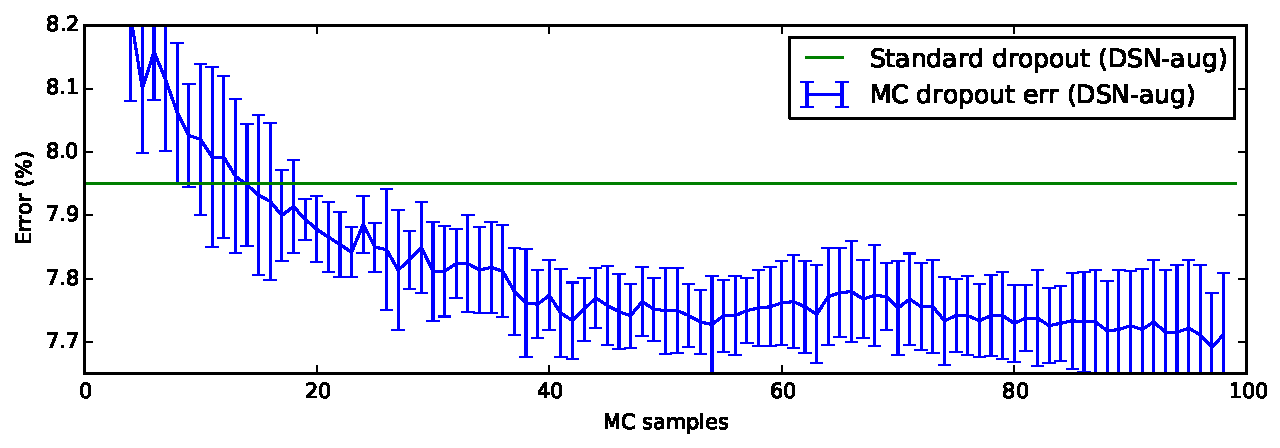
\includegraphics[width=1.0\textwidth]{uncertainty/DSN_samples}
		\caption{Ovisnost klasifikacijske pogreške (plavo) o broju uzoraka u \textit{Monte Carlo} aproksimaciji izlaza na konvolucijskoj mreži koju su ispitivali autori \citep{Gal:2016:BCNNBAVI} na skupu CIFAR-10. Svaka točka je prosjek $5$ mjerenja i prikazane su standardne devijacije. Zeleni pravac označava klasifikacijsku pogrešku kod userdnjavanja kakvo se inače koristi kod testiranja. Slika je preuzeta iz \citet{Gal:2016:BCNNBAVI}.}
		\label{fig:mc-drouput-samples-DSN}
	\end{figure}
\end{frame}


\begin{frame}[allowframebreaks=0.9]{Prepoznavanje izvanrazdiobnih i krivo klasificiranih primjera na temelju izlaza softmaksa ili logita}
\begin{itemize}
	\item Razdiobe koje duboki modeli daju kao izlaz softmaksa su često previše sigurne kod krive klasifikacije i nije ih dobro interpretirati kao vjerojatnosti.
	\item \citet{Hendrycks:2016:BDMOODE} pokazuju da se krivo klasificirani i izvanrazdiobni primjeri ipak mogu uspješno prepoznavati klasifikacijom maksimalne vjerojatnosti softmaksa. 
	\item \citet{Guo:2017:CMNN} pokazuju da se \textbf{temperaturnim skaliranjem} softmaksa može značajno poboljšati kalibracija izlazne razdiobe već naučene mreže. Kod temperaturnog skaliranja, ako su logiti $\vec s$ ($h(\vec x)=\softmax(\vec s)$), izlazni vektor vjerojatnosti uz temperaturno skaliranje je $\softmax\del{\frac{1}{T}\vec s}$.	
	\item \citet{Liang:2017:PDOODENN} predlažu $2$ poboljšanja klasifikacije maksimalne vrijednosti softmaksa za prepoznavanje izvanrazdiobnih primjera. Jedno poboljšanje je temperaturno skaliranje. Pokazuju da, što je veća temperatura, to se izvanrazdiobni primjeri mogu bolje odvojiti od unutarrazdiobnih primjera na temelju maksimalne vrijednosti softmaksa. Drugo poboljšanje je izmjena ulaza mreže tako da se \textbf{FGSM-om} pomakne u smjeru povećavanja maksimalnog izlaza softmaksa:
	\begin{equation} \label{eq:ODIN-FGSM}
	\tilde{\vec x} = \vec x - \epsilon\sgn\nabla_{\vec x}\del{-\ln \max_k \p(\rvar y=k\mid x,\vec\theta)} \text{.}
	\end{equation}
	$\epsilon$ je parametar koji se određuje pomoću izdvojenog podskupa izvanrazdiobnih primjera.		
	\item Za ovaj rad su još ispitani neki slični pristupi kod kojih se umjesto maksimalnog izlaza softmaksa za prepoznavanje izvanrazdiobnih primjera koristi maksimalni logit ili neke druge značajke izvedene iz vektora logita.
\end{itemize}
\end{frame}


\section{Eksperimenti}

\begin{frame}[allowframebreaks=0.9]{Procjena i razlikovanje nesigurnosti kod semantičke segmentacije pomoću dropouta}
\begin{itemize}
	\item 
\end{itemize}
\end{frame}

\begin{frame}[allowframebreaks=0.9]
\frametitle{Literatura}
	\bibliography{literatura}
	\bibliographystyle{fer} 
\end{frame}

\end{document}
